\documentclass[aspectratio=169,10pt]{beamer}

\usepackage{fontspec}
\usepackage{lmodern}
\usepackage{amsmath,amssymb,mathtools}
\usepackage{booktabs,tabularx,array}
\usepackage{tikz}
\usetikzlibrary{positioning}
\usepackage{fancyvrb}
\usepackage{hyperref}
\usepackage{ragged2e}

\setmonofont{DejaVuSansMono.ttf}[
  Path=/usr/local/texlive/2024/texmf-dist/fonts/truetype/public/dejavu/]
\renewcommand{\familydefault}{\sfdefault}

\definecolor{DOneBackground}{RGB}{251,252,248}
\definecolor{DOnePanel}{RGB}{243,248,255}
\definecolor{DOneCode}{RGB}{247,250,253}
\definecolor{DOneInk}{RGB}{19,32,43}
\definecolor{DOneBlue}{RGB}{8,62,117}
\definecolor{DOneBrightBlue}{RGB}{11,92,173}
\definecolor{DOneMuted}{RGB}{91,103,122}
\definecolor{DOneLine}{RGB}{184,204,229}
\definecolor{DOneGreen}{RGB}{38,111,78}
\definecolor{DOneRed}{RGB}{163,58,58}
\definecolor{DOneAmber}{RGB}{145,95,16}

\setbeamercolor{normal text}{fg=DOneInk,bg=DOneBackground}
\setbeamercolor{structure}{fg=DOneBrightBlue}
\setbeamercolor{frametitle}{fg=DOneBlue,bg=DOneBackground}
\setbeamercolor{panel}{fg=DOneInk,bg=DOnePanel}
\setbeamercolor{code box}{fg=DOneInk,bg=DOneCode}
\setbeamercolor{alerted text}{fg=DOneRed}

\setbeamerfont{frametitle}{size=\Large,series=\bfseries}
\setbeamerfont{normal text}{size=\normalsize}
\setbeamerfont{footline}{size=\fontsize{5.7}{6.5}\selectfont}
\setbeamertemplate{navigation symbols}{}
\setbeamertemplate{itemize item}{\color{DOneBrightBlue}\raise0.15ex\hbox{\scriptsize$\blacktriangleright$}}
\setbeamertemplate{itemize subitem}{\color{DOneBrightBlue}\raise0.15ex\hbox{\tiny$\blacktriangleright$}}
\setbeamertemplate{enumerate item}{\color{DOneBlue}\insertenumlabel.}
\setbeamertemplate{frametitle}{%
  \nointerlineskip
  \vspace{0.18cm}
  \hspace{0.14cm}\insertframetitle\par
  \vspace{0.08cm}
}
\setbeamertemplate{footline}{%
  \leavevmode
  \hbox{%
    \begin{beamercolorbox}[wd=.33\paperwidth,ht=0.35cm,dp=0.13cm,leftskip=0.48cm]{normal text}%
      \color{DOneMuted}\usebeamerfont{footline}\insertsectionhead
    \end{beamercolorbox}%
    \begin{beamercolorbox}[wd=.34\paperwidth,ht=0.35cm,dp=0.13cm,center]{normal text}%
      \color{DOneMuted}\usebeamerfont{footline}D3: Lean and AI
    \end{beamercolorbox}%
    \begin{beamercolorbox}[wd=.33\paperwidth,ht=0.35cm,dp=0.13cm,rightskip=0.48cm plus1fil]{normal text}%
      \color{DOneMuted}\usebeamerfont{footline}\insertframenumber\ / \inserttotalframenumber
    \end{beamercolorbox}%
  }
}

\setbeamersize{text margin left=0.62cm,text margin right=0.62cm}
\setlength{\tabcolsep}{5pt}
\renewcommand{\arraystretch}{1.15}
\hypersetup{colorlinks=true,linkcolor=DOneBrightBlue,urlcolor=DOneBrightBlue}

\newcommand{\term}[1]{\textcolor{DOneBlue}{\textbf{#1}}}
\newcommand{\muted}[1]{\textcolor{DOneMuted}{#1}}
\newcommand{\good}[1]{\textcolor{DOneGreen}{\textbf{#1}}}
\newcommand{\bad}[1]{\textcolor{DOneRed}{\textbf{#1}}}
\newcommand{\livelean}[1]{%
  \vspace{0.08cm}\par{\scriptsize\color{DOneMuted}%
  Live Lean: \href{run:#1}{\nolinkurl{#1}}}%
}
\newcommand{\schematic}{%
  \vspace{0.08cm}\par{\scriptsize\color{DOneMuted}%
  \textbf{Not copy-paste Lean code; schematic extract only.} Universes, implicit parameters, and some inherited fields are omitted.}%
}
\newcommand{\coreextract}{%
  \vspace{0.04cm}\par{\scriptsize\color{DOneMuted}%
  Core fields from the current Mathlib hierarchy; documentation, universes, and default proof bodies are omitted.}%
}
\newenvironment{dpanel}{%
  \begin{beamercolorbox}[wd=\dimexpr\linewidth-9pt\relax,leftskip=0.15cm,rightskip=0.15cm plus1fil,rounded=true]{panel}%
  \setlength{\linewidth}{\hsize}%
  \vspace{0.10cm}%
}{\vspace{0.10cm}\end{beamercolorbox}}
\newenvironment{leancode}{%
  \VerbatimEnvironment
  \begin{beamercolorbox}[wd=\linewidth,leftskip=0.10cm,rightskip=0.10cm plus1fil,rounded=false]{code box}%
  \setlength{\linewidth}{\hsize}%
  \vspace{0.06cm}%
  \begin{Verbatim}[fontsize=\scriptsize,formatcom=\color{DOneInk}]%
}{%
  \end{Verbatim}
  \vspace{0.06cm}\end{beamercolorbox}%
}
\newenvironment{leancodesmall}{%
  \VerbatimEnvironment
  \begin{beamercolorbox}[wd=\linewidth,leftskip=0.10cm,rightskip=0.10cm plus1fil,rounded=false]{code box}%
  \setlength{\linewidth}{\hsize}%
  \vspace{0.05cm}%
  \begin{Verbatim}[fontsize=\fontsize{6.8}{7.7}\selectfont,formatcom=\color{DOneInk}]%
}{%
  \end{Verbatim}
  \vspace{0.05cm}\end{beamercolorbox}%
}
\newcolumntype{Y}{>{\RaggedRight\arraybackslash}X}
\newcolumntype{B}{>{\RaggedRight\arraybackslash\bfseries\color{DOneBlue}}p{0.22\linewidth}}

\title{Lean and AI}
\subtitle{From algebraic instances to kernel-checked formalization}
\author{AI4Math Summer School}
\date{}

\begin{document}

\section{Overview}

\begin{frame}[plain]
  
\begin{tikzpicture}[remember picture,overlay]
    \node[anchor=north west,text=DOneBlue,font=\fontsize{10}{12}\selectfont]
      at ([xshift=0.95cm,yshift=-0.62cm]current page.north west)
      {AI4Math Summer School $\cdot$ D3};
    \node[anchor=north west,text=DOneInk,font=\bfseries\fontsize{25}{29}\selectfont]
      at ([xshift=0.95cm,yshift=-1.72cm]current page.north west)
      {Lean and AI};
    \node[anchor=north west,text=DOneMuted,font=\bfseries\fontsize{15}{18}\selectfont]
      at ([xshift=0.95cm,yshift=-2.65cm]current page.north west)
      {From algebraic instances to kernel-checked formalization};
    \fill[rounded corners=5pt,DOnePanel]
      ([xshift=0.82cm,yshift=0.72cm]current page.south west)
      rectangle ([xshift=9.22cm,yshift=3.36cm]current page.south west);
    \node[anchor=north west,text=DOneBlue,font=\bfseries\fontsize{11}{13}\selectfont]
      at ([xshift=1.25cm,yshift=3.05cm]current page.south west) {Today’s route};
    \node[anchor=north west,text=DOneInk,align=left,text width=7.45cm,font=\fontsize{9.8}{12}\selectfont]
      at ([xshift=1.25cm,yshift=2.55cm]current page.south west)
      {Algebraic hierarchy $\rightarrow$ substructures $\rightarrow$ modules and choice\\[2pt]
       Categories and complexes $\rightarrow$ AI-assisted Lean\\[2pt]
       Finite counting and graphs};
    \node[anchor=north west,text=DOneInk,font=\bfseries\fontsize{10}{12}\selectfont]
      at ([xshift=9.9cm,yshift=3.05cm]current page.south west) {Three-hour session};
    \node[anchor=north west,text=DOneInk,align=left,font=\fontsize{9.8}{12}\selectfont]
      at ([xshift=9.9cm,yshift=2.55cm]current page.south west)
      {Instances, Mathlib search,\\research-level interfaces,\\and AI failure analysis.};
  \end{tikzpicture}
\end{frame}

\begin{frame}{Learning Goals}
\begin{columns}[T,onlytextwidth]
  \column{0.49\textwidth}
  \begin{dpanel}
  \term{Read algebraic interfaces}\\
  Explain what \texttt{AddGroup}, \texttt{Group}, \texttt{Ring}, \texttt{Field}, and \texttt{Module} require.
  \end{dpanel}
  \vspace{0.17cm}
  \begin{dpanel}
  \term{Build and inspect instances}\\
  Separate operation fields from law fields; diagnose typeclass search with \texttt{\#synth} and \texttt{\#check}.
  \end{dpanel}
  \vspace{0.17cm}
  \begin{dpanel}
  \term{Use substructures}\\
  Read subtype elements and construct subgroups, subrings, and submodules by closure proofs.
  \end{dpanel}
  \column{0.49\textwidth}
  \begin{dpanel}
  \term{See research-level interfaces}\\
  Recognize categories, functors, natural transformations, and homological complexes in Mathlib.
  \end{dpanel}
  \vspace{0.17cm}
  \begin{dpanel}
  \term{Formalize finite mathematics}\\
  Use \texttt{Finset}, \texttt{SimpleGraph}, \texttt{simp}, \texttt{ring}, \texttt{linarith}, and \texttt{decide}.
  \end{dpanel}
  \vspace{0.17cm}
  \begin{dpanel}
  \term{Use AI critically}\\
  Let AI propose statements and proofs, then verify semantics, API names, assumptions, and kernel acceptance.
  \end{dpanel}
\end{columns}
\end{frame}

\section{Part I: Algebraic Structures}

\begin{frame}[fragile]{An Instance Is Lean’s Entry Point to Structure}
\begin{columns}[T,onlytextwidth]
  \column{0.32\textwidth}
  \begin{dpanel}\centering
  \term{Object}\\[3pt]
  \texttt{G : Type*}\\
  only gives a type
  \end{dpanel}
  \column{0.32\textwidth}
  \begin{dpanel}\centering
  \term{Structure}\\[3pt]
  \texttt{[Group G]}\\
  asks typeclass search
  \end{dpanel}
  \column{0.32\textwidth}
  \begin{dpanel}\centering
  \term{Theorems}\\[3pt]
  \texttt{mul\_assoc}\\
  becomes available
  \end{dpanel}
\end{columns}
\vspace{0.32cm}
\begin{leancode}
variable (G : Type*) [Group G]

#synth Group G
#check mul_assoc
#check inv_mul_cancel
\end{leancode}
\vspace{0.15cm}
Parentheses introduce ordinary arguments. Square brackets introduce arguments that Lean should synthesize automatically.
\vspace{0.08cm}

{\scriptsize\color{DOneMuted}\textbf{Environment:} Open and run these files inside a configured Mathlib Lake project. The distributed D3 folder alone is not a Lake project.}
\livelean{D3_01_Inspect.lean}
\end{frame}

\begin{frame}{Writing an Instance: Data First, Laws Second}
\begin{columns}[T,onlytextwidth]
  \column{0.49\textwidth}
  \begin{dpanel}
  \term{Operation data}
  \begin{itemize}
    \item \texttt{mul}, \texttt{one}, \texttt{inv}
    \item \texttt{add}, \texttt{zero}, \texttt{neg}
    \item \texttt{Hom}, \texttt{id}, \texttt{comp}
  \end{itemize}
  These fields determine what notation means.
  \end{dpanel}
  \column{0.49\textwidth}
  \begin{dpanel}
  \term{Proof data}
  \begin{itemize}
    \item associativity, identities, inverses
    \item distributivity and commutativity
    \item category identity and associativity laws
  \end{itemize}
  Every law is a separate Lean goal.
  \end{dpanel}
\end{columns}
\vspace{0.35cm}
\begin{dpanel}
\term{Practical inspection loop:} use \texttt{\#print} to inspect fields; write a field followed by \texttt{:= by}; read the new goal; prove it; continue to the next field.
\end{dpanel}
\end{frame}

\begin{frame}[fragile]{\texttt{extends} Reuses a Parent Interface}
\begin{columns}[T,onlytextwidth]
\column{0.62\textwidth}
\begin{leancodesmall}
class Add (G : Type u) where
  add : G → G → G

class AddSemigroup (G : Type u)
    extends Add G where
  protected add_assoc : ∀ a b c : G,
    a + b + c = a + (b + c)

variable (G : Type*) [AddSemigroup G]
#synth Add G
#check AddSemigroup.toAdd
\end{leancodesmall}
\column{0.35\textwidth}
\begin{dpanel}
\term{What \texttt{extends} does}
\begin{itemize}
  \item inherits the fields of \texttt{Add G}
  \item adds the new field \texttt{add\_assoc}
  \item creates a parent projection
  \item lets typeclass search use the child as the parent
  \item does not prove the new law
\end{itemize}
\end{dpanel}
\end{columns}
\vspace{0.10cm}
\begin{dpanel}
\term{Multiple inheritance:} \texttt{AddMonoid G extends AddSemigroup G, AddZeroClass G}. An \texttt{AddMonoid G} can be used through either parent interface, but an \texttt{Add G} alone cannot be promoted to either child.
\end{dpanel}
\livelean{D3_02_AddGroup_Group.lean}
\end{frame}

\begin{frame}{The Actual Mathlib Path from Add to AddGroup}
\centering
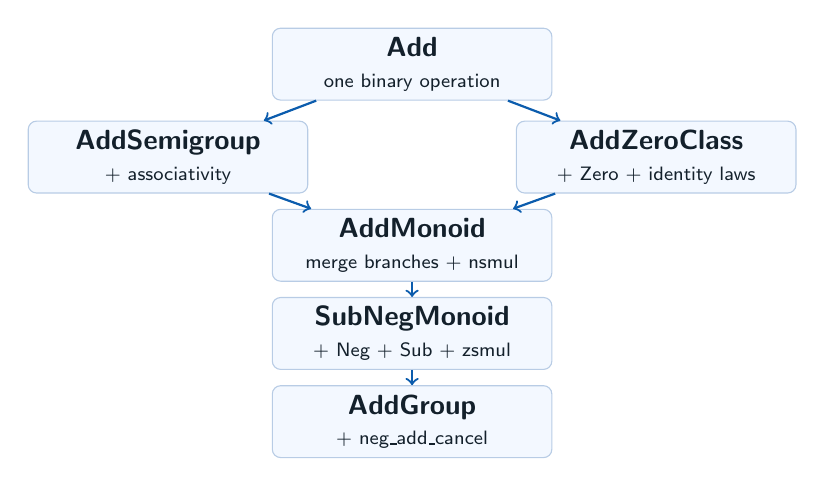
\begin{tikzpicture}[
  box/.style={draw=DOneLine,fill=DOnePanel,rounded corners=3pt,minimum width=3.55cm,minimum height=0.68cm,text=DOneInk,align=center},
  arr/.style={->,thick,draw=DOneBrightBlue}]
  \node[box] (add) at (0,0) {\textbf{Add}\\[-1pt]{\scriptsize one binary operation}};
  \node[box] (semigroup) at (-3.1,-1.18) {\textbf{AddSemigroup}\\[-1pt]{\scriptsize + associativity}};
  \node[box] (zeroclass) at (3.1,-1.18) {\textbf{AddZeroClass}\\[-1pt]{\scriptsize + Zero + identity laws}};
  \node[box] (monoid) at (0,-2.30) {\textbf{AddMonoid}\\[-1pt]{\scriptsize merge branches + nsmul}};
  \node[box] (subneg) at (0,-3.42) {\textbf{SubNegMonoid}\\[-1pt]{\scriptsize + Neg + Sub + zsmul}};
  \node[box] (group) at (0,-4.54) {\textbf{AddGroup}\\[-1pt]{\scriptsize + neg\_add\_cancel}};
  \draw[arr] (add)--(semigroup);
  \draw[arr] (add)--(zeroclass);
  \draw[arr] (semigroup)--(monoid);
  \draw[arr] (zeroclass)--(monoid);
  \draw[arr] (monoid)--(subneg);
  \draw[arr] (subneg)--(group);
\end{tikzpicture}
\vspace{0.06cm}
\begin{dpanel}
\term{Two branches merge at AddMonoid.} Associativity comes from \texttt{AddSemigroup}; zero and its identity laws come from \texttt{AddZeroClass}. Negation does not become an additive inverse until the final \texttt{AddGroup} axiom is proved.
\end{dpanel}
\end{frame}

\begin{frame}[fragile]{Step 0: Add Supplies an Operation, Not a Law}
\begin{columns}[T,onlytextwidth]
\column{0.66\textwidth}
\begin{leancode}
class Add (G : Type u) where
  add : G → G → G

class AddSemigroup (G : Type u)
    extends Add G where
  protected add_assoc : ∀ a b c : G,
    a + b + c = a + (b + c)
\end{leancode}
\column{0.31\textwidth}
\begin{dpanel}
\term{After Add}
\begin{itemize}
  \item Lean can elaborate \texttt{a + b}.
  \item No theorem relates different sums.
  \item Even \texttt{(a+b)+c = a+(b+c)} is unavailable.
\end{itemize}
\end{dpanel}
\vspace{0.2cm}
\begin{dpanel}
\term{AddSemigroup adds exactly one mathematical law:} associativity.
\end{dpanel}
\end{columns}
\coreextract
\livelean{D3_02_AddGroup_Group.lean}
\end{frame}

\begin{frame}[fragile]{Step 1: Add Zero and Merge the Two Branches}
\begin{columns}[T,onlytextwidth]
\column{0.69\textwidth}
\begin{leancodesmall}
class AddZero (G : Type u) extends Zero G, Add G

class AddZeroClass (G : Type u)
    extends AddZero G where
  protected zero_add : ∀ a : G, 0 + a = a
  protected add_zero : ∀ a : G, a + 0 = a

class AddMonoid (G : Type u)
    extends AddSemigroup G, AddZeroClass G where
  protected nsmul : ℕ → G → G
  protected nsmul_zero : ∀ x, nsmul 0 x = 0
  protected nsmul_succ : ∀ n x,
    nsmul (n + 1) x = nsmul n x + x
\end{leancodesmall}
\column{0.28\textwidth}
\begin{dpanel}
\term{Why three classes?}
\begin{itemize}
  \item \texttt{AddZero}: data only
  \item \texttt{AddZeroClass}: zero laws
  \item \texttt{AddMonoid}: also associativity
  \item \texttt{nsmul}: interprets \texttt{n • a}
\end{itemize}
\end{dpanel}
\vspace{0.2cm}
Natural scalar multiplication is an engineering field with a standard default implementation.
\end{columns}
\coreextract
\livelean{D3_02_AddGroup_Group.lean}
\end{frame}

\begin{frame}[fragile]{\texttt{nsmul}: Repeated Addition by a Natural Number}
\begin{columns}[T,onlytextwidth]
\column{0.58\textwidth}
\begin{leancodesmall}
class AddMonoid (M : Type u) where
  protected nsmul : ℕ → M → M
  protected nsmul_zero : ∀ a,
    nsmul 0 a = 0
  protected nsmul_succ : ∀ n a,
    nsmul (n + 1) a = nsmul n a + a
\end{leancodesmall}
\vspace{0.12cm}
\begin{leancodesmall}
variable (M : Type*) [AddMonoid M]
#synth SMul ℕ M
#check zero_nsmul
#check succ_nsmul

example : (3 : ℕ) • (5 : ℤ) = 15 := by
  norm_num
\end{leancodesmall}
\column{0.39\textwidth}
\begin{dpanel}
\term{Mathematical meaning}
\begin{itemize}
  \item \texttt{0 • a = 0}
  \item \texttt{(n+1) • a = n • a + a}
  \item hence \texttt{n • a} is (n) copies of (a)
\end{itemize}
\vspace{0.05cm}
\term{Why it is needed}
\begin{itemize}
  \item gives \texttt{SMul ℕ M} to every additive monoid
  \item enables \texttt{n • a} in algebraic statements
  \item stores one operation to avoid instance diamonds
\end{itemize}
\end{dpanel}
\end{columns}
\coreextract
\livelean{D3_02_AddGroup_Group.lean}
\end{frame}

\begin{frame}[fragile]{Step 2: SubNegMonoid Adds Syntax for Negation and Subtraction}
\begin{columns}[T,onlytextwidth]
\column{0.69\textwidth}
\begin{leancodesmall}
class SubNegMonoid (G : Type u)
    extends AddMonoid G, Neg G, Sub G where
  protected sub : G → G → G :=
    fun a b => a + -b
  protected sub_eq_add_neg : ∀ a b : G,
    a - b = a + -b
  protected zsmul : ℤ → G → G
  protected zsmul_zero' : ∀ a, zsmul 0 a = 0
  protected zsmul_succ' : ∀ n a,
    zsmul n.succ a = zsmul n a + a
  protected zsmul_neg' : ∀ n a,
    zsmul (Int.negSucc n) a = -zsmul n.succ a
\end{leancodesmall}
\column{0.28\textwidth}
\begin{dpanel}
\small
\term{Important distinction}
\begin{itemize}
  \item \texttt{Neg G} only defines \texttt{-a}.
  \item \texttt{Sub G} only defines \texttt{a-b}.
  \item \texttt{sub\_eq\_add\_neg} connects the notations.
  \item \texttt{zsmul} gives integer scalar multiplication.
  \item No inverse law has been required yet.
\end{itemize}
\end{dpanel}
\end{columns}
\livelean{D3_02_AddGroup_Group.lean}
\end{frame}

\begin{frame}[fragile]{\texttt{nsmul} and \texttt{zsmul}: Two Natural Interfaces}
\begin{columns}[T,onlytextwidth]
\column{0.61\textwidth}
\begin{leancodesmall}
class NsmulData (α : Type u) where
  nsmul : ℕ → α → α

class ZsmulData (α : Type u) where
  zsmul : ℤ → α → α

-- two mathematically natural definitions
n • x := x + x + ⋯ + x       -- n times
n • x := (n : ℤ) • x          -- restrict zsmul to ℕ
\end{leancodesmall}
\column{0.34\textwidth}
\begin{dpanel}
\term{The mathematics}
\begin{itemize}
  \item both definitions express repeated addition
  \item negative integers use \texttt{-x}
  \item under the intended laws, they should agree
\end{itemize}
\vspace{0.10cm}
\term{The Lean question}
Which operation is the actual data behind \texttt{n • x}? If two instance paths construct it, the definitions may be mathematically equal without being definitionally equal.
\end{dpanel}
\end{columns}
\schematic
\livelean{D3_02_AddGroup_Group.lean}
\end{frame}

\begin{frame}[fragile]{A Bad Hierarchy Creates Two \texttt{nsmul} Paths}
\begin{columns}[T,onlytextwidth]
\column{0.62\textwidth}
\begin{leancodesmall}
class BadAddMonoid (α : Type u)
    extends Add α, Zero α, NsmulData α

class BadAddGroup (α : Type u)
    extends Add α, Zero α, Neg α

instance groupToMonoid [BadAddGroup α] : BadAddMonoid α where
  nsmul := repeatedAddition

instance groupToZsmul [BadAddGroup α] : ZsmulData α where
  zsmul := integerRepeatedAddition

instance nsmulFromZsmul [ZsmulData α] : NsmulData α where
  nsmul n x := ZsmulData.zsmul (n : ℤ) x
\end{leancodesmall}
\column{0.33\textwidth}
\centering
\begin{tikzpicture}[
  box/.style={draw=DOneLine,fill=DOnePanel,rounded corners=3pt,minimum width=1.85cm,minimum height=0.58cm,font=\fontsize{5.8}{6.5}\selectfont,text=DOneInk,align=center},
  arr/.style={->,thick,draw=DOneBrightBlue}]
  \node[box] (g) at (0,0) {\texttt{BadAddGroup α}};
  \node[box] (m) at (-1.05,-1.1) {\texttt{BadAddMonoid}};
  \node[box] (z) at (1.05,-1.1) {\texttt{ZsmulData}};
  \node[box] (n) at (0,-2.2) {\texttt{NsmulData α}};
  \draw[arr] (g)--(m);
  \draw[arr] (g)--(z);
  \draw[arr] (m)--(n);
  \draw[arr] (z)--(n);
\end{tikzpicture}
\vspace{0.10cm}
\begin{dpanel}
\small
There are two routes from \texttt{BadAddGroup α} to the same target instance.
Priority can select one route, but it does not make the operations coherent.
\end{dpanel}
\end{columns}
\schematic
\livelean{D3_02_AddGroup_Group.lean}
\end{frame}

\begin{frame}[fragile]{Why the Diamond Needs Definitional Equality}
\begin{columns}[T,onlytextwidth]
\column{0.57\textwidth}
\begin{leancodesmall}
-- the same expression, reached by two paths
-- Path A: 2 • x  ↦  x + (x + 0)
-- Path B: 2 • x  ↦  (2 : ℤ) • x
--              ↦  zsmulRec (2 : ℤ) x

-- Mathlib's actual scalar operation
#synth SMul ℕ (Polynomial ℕ)
example (n : ℕ) (p : Polynomial ℕ) :
    AddMonoid.nsmul n p = n • p := by
  rfl
\end{leancodesmall}
\column{0.40\textwidth}
\begin{dpanel}
\small
\term{Two notions of equality}
\begin{itemize}
  \item propositional: needs a proof and possibly \texttt{rw}
  \item definitional: both terms reduce to the same expression; \texttt{rfl} works
\end{itemize}
\vspace{0.05cm}
\term{Mathlib's fix}
\begin{itemize}
  \item \texttt{nsmul} is stored in \texttt{AddMonoid}
  \item \texttt{zsmul} is stored in \texttt{SubNegMonoid}, the parent of \texttt{AddGroup}
  \item \texttt{SMul} projects these fixed fields
\end{itemize}
\good{All paths reuse fixed fields.}
\end{dpanel}
\end{columns}
\coreextract
\livelean{D3_02_AddGroup_Group.lean}
\end{frame}

\begin{frame}[fragile]{Step 3: AddGroup Adds the Inverse Axiom}
\begin{columns}[T,onlytextwidth]
\column{0.58\textwidth}
\begin{leancode}
class AddGroup (G : Type u)
    extends SubNegMonoid G where
  protected neg_add_cancel : ∀ a : G,
    -a + a = 0
\end{leancode}
\vspace{0.22cm}
\begin{leancode}
#check neg_add_cancel
#check add_neg_cancel
#check sub_self
#check neg_add_rev
#check add_left_cancel
\end{leancode}
\column{0.39\textwidth}
\begin{dpanel}
\term{Only one new axiom is stored.} Mathlib derives:
\begin{itemize}
  \item the right inverse law \texttt{a + -a = 0}
  \item cancellation laws
  \item \texttt{a - a = 0}
  \item involutive negation
  \item negation reversing addition
\end{itemize}
\end{dpanel}
\vspace{0.2cm}
Typeclass search also synthesizes \texttt{AddCancelMonoid} and \texttt{SubtractionMonoid}.
\end{columns}
\coreextract
\livelean{D3_02_AddGroup_Group.lean}
\end{frame}

\begin{frame}[fragile]{Practical Construction: First Provide Add, Zero, and Neg}
\begin{columns}[T,onlytextwidth]
\column{0.66\textwidth}
\begin{leancode}
@[ext]
structure WrappedInt where
  val : ℤ

instance : Add WrappedInt where
  add a b := ⟨a.val + b.val⟩

instance : Zero WrappedInt where
  zero := ⟨0⟩

instance : Neg WrappedInt where
  neg a := ⟨-a.val⟩

#synth Add WrappedInt
-- #synth AddGroup WrappedInt  -- not yet
\end{leancode}
\column{0.31\textwidth}
\begin{dpanel}
\term{At this point Lean knows only the operations.}
\begin{itemize}
  \item \texttt{a + b} unwraps, adds integers, and wraps again.
  \item \texttt{0} wraps integer zero.
  \item \texttt{-a} wraps integer negation.
  \item No group theorem is available yet.
\end{itemize}
\end{dpanel}
\end{columns}
\livelean{D3_02_AddGroup_Group.lean}
\end{frame}

\begin{frame}[fragile]{AddGroup.ofLeftAxioms Builds the Full Instance}
\begin{columns}[T,onlytextwidth]
\column{0.69\textwidth}
\begin{leancodesmall}
instance : AddGroup WrappedInt :=
  AddGroup.ofLeftAxioms
    (fun a b c => by
      apply WrappedInt.ext
      exact add_assoc a.val b.val c.val)
    (fun a => by
      apply WrappedInt.ext
      exact zero_add a.val)
    (fun a => by
      apply WrappedInt.ext
      exact neg_add_cancel a.val)

#synth AddMonoid WrappedInt
#synth SubNegMonoid WrappedInt
#synth AddGroup WrappedInt
#synth AddCancelMonoid WrappedInt
\end{leancodesmall}
\column{0.28\textwidth}
\begin{dpanel}
\term{Only three proofs}
\begin{enumerate}
  \item associativity
  \item left zero law
  \item left inverse law
\end{enumerate}
\end{dpanel}
\vspace{0.22cm}
The constructor supplies default \texttt{sub}, \texttt{nsmul}, and \texttt{zsmul}, and derives the remaining group laws.
\end{columns}
\livelean{D3_02_AddGroup_Group.lean}
\end{frame}

\begin{frame}[fragile]{AddGroup and Group: Same Pattern, Different Interface}
\begin{dpanel}
\begin{tabularx}{\linewidth}{@{}B Y Y@{}}
\toprule
Structure & Notation and data & Core laws \\
\midrule
\texttt{AddGroup A} & \texttt{0}, \texttt{+}, \texttt{-a} & additive associativity, zero laws, additive inverse \\
\texttt{Group G} & \texttt{1}, \texttt{*}, \texttt{g⁻¹} & multiplicative associativity, identity laws, multiplicative inverse \\
\bottomrule
\end{tabularx}
\end{dpanel}
\vspace{0.12cm}
\begin{leancode}
example (A : Type*) [AddGroup A] (a : A) :
    -a + a = 0 := neg_add_cancel a

example (G : Type*) [Group G] (g : G) :
    g⁻¹ * g = 1 := inv_mul_cancel g
\end{leancode}
\vspace{0.05cm}
They are distinct classes. Mathlib relates many parallel theorems through \texttt{to\_additive}; notation still determines the interface Lean searches for.
\livelean{D3_02_AddGroup_Group.lean}
\end{frame}

\begin{frame}[fragile]{The \texttt{Group} Class in Mathlib}
\begin{columns}[T,onlytextwidth]
\column{0.67\textwidth}
\begin{leancodesmall}
class DivInvMonoid (G : Type u)
    extends Monoid G, Inv G, Div G where
  protected div_eq_mul_inv : ∀ a b : G,
    a / b = a * b⁻¹

class Group (G : Type u)
    extends DivInvMonoid G where
  protected inv_mul_cancel : ∀ a : G,
    a⁻¹ * a = 1
\end{leancodesmall}
\column{0.29\textwidth}
\begin{dpanel}
\term{Parent chain}
\begin{itemize}
  \item \texttt{Monoid}: \texttt{*}, \texttt{1}, monoid laws
  \item \texttt{DivInvMonoid}: \texttt{⁻¹}, \texttt{/}, compatible division
  \item \texttt{Group}: stored law \texttt{a⁻¹*a = 1}
\end{itemize}
\end{dpanel}
\end{columns}
\vspace{0.05cm}
\begin{leancodesmall}
variable (G : Type*) [Group G]
#synth Monoid G
#synth DivInvMonoid G
#check Group.toDivInvMonoid
#check Group.inv_mul_cancel     -- stored field
#check inv_mul_cancel            -- public theorem
\end{leancodesmall}
\coreextract
\livelean{D3_02_AddGroup_Group.lean}
\end{frame}

\begin{frame}[fragile]{Why AddGroup Appears Before Linear Algebra}
\begin{columns}[T,onlytextwidth]
\column{0.49\textwidth}
\begin{dpanel}
\term{Group-theoretic language}
\begin{itemize}
  \item \texttt{[Group G]} gives a multiplicative group.
  \item Theorems use \texttt{a * b} and \texttt{a⁻¹}.
  \item Order matters in noncommutative groups.
\end{itemize}
\end{dpanel}
\column{0.49\textwidth}
\begin{dpanel}
\term{Linear-algebra language}
\begin{itemize}
  \item \texttt{[AddCommGroup V]} gives vector addition.
  \item A module adds scalar multiplication \texttt{r • v}.
  \item Vector spaces use the additive interface.
\end{itemize}
\end{dpanel}
\end{columns}
\vspace{0.30cm}
\begin{leancode}
#check add_assoc       -- additive interface
#check mul_assoc       -- multiplicative interface
#check neg_add_cancel  -- AddGroup
#check inv_mul_cancel  -- Group
\end{leancode}
\end{frame}

\begin{frame}[fragile]{Example: Define the Operations of the Sign Group}
\begin{columns}[T,onlytextwidth]
\column{0.66\textwidth}
\begin{leancode}
inductive Sign where
  | pos
  | neg
  deriving DecidableEq, Repr

open Sign

instance : Group Sign where
  mul a b :=
    match a, b with
    | pos, x => x
    | neg, pos => neg
    | neg, neg => pos
  one := pos
  inv a := a
  -- law fields come next
\end{leancode}
\column{0.31\textwidth}
\begin{dpanel}
\term{Mathematical reading}
\begin{itemize}
  \item \texttt{pos} is the identity.
  \item \texttt{neg * neg = pos}.
  \item Every element is self-inverse.
\end{itemize}
\end{dpanel}
\vspace{0.2cm}
First define the table. Then let Lean expose one law goal at a time.
\end{columns}
\livelean{D3_04_Group_Instance.lean}
\end{frame}

\begin{frame}[fragile]{Check the Group Laws One by One}
\begin{columns}[T,onlytextwidth]
\column{0.63\textwidth}
\begin{leancode}
  mul_assoc := by
    intro a b c
    cases a <;> cases b <;> cases c <;> rfl

  one_mul := by
    intro a
    cases a <;> rfl

  mul_one := by
    intro a
    cases a <;> rfl

  inv_mul_cancel := by
    intro a
    cases a <;> rfl
\end{leancode}
\column{0.34\textwidth}
\begin{dpanel}
\term{What Lean checks}
\begin{enumerate}
  \item \texttt{intro} exposes arbitrary elements.
  \item \texttt{cases} enumerates \texttt{pos}/\texttt{neg}.
  \item \texttt{rfl} checks the reduced definitions.
\end{enumerate}
\end{dpanel}
\vspace{0.22cm}
\begin{leancode}
#synth Group Sign

example (a : Sign) :
    a⁻¹ * a = 1 :=
  inv_mul_cancel a
\end{leancode}
\end{columns}
\end{frame}

\section{Part II: Subtypes and Substructures}

\begin{frame}[fragile]{Subtype: A Value Packaged with a Proof}
\begin{columns}[T,onlytextwidth]
\column{0.64\textwidth}
\begin{leancode}
def NonzeroInt := {n : ℤ // n ≠ 0}

example : NonzeroInt :=
  ⟨1, by norm_num⟩

example (x : NonzeroInt) : ℤ :=
  x.1

example (x : NonzeroInt) : x.1 ≠ 0 :=
  x.property

#check Subtype.val
#check Subtype.property
\end{leancode}
\column{0.33\textwidth}
\begin{dpanel}
\term{How to read it}
\begin{itemize}
  \item \texttt{x.1} is the underlying value.
  \item \texttt{x.2} or \texttt{x.property} is the proof.
  \item \texttt{⟨value, proof⟩} constructs an element.
\end{itemize}
\end{dpanel}
\vspace{0.25cm}
Subgroups, subrings, and submodules all reuse this pattern.
\end{columns}
\livelean{D3_03_Subtype.lean}
\end{frame}

\begin{frame}[fragile]{Subgroup = Carrier Predicate + Closure Proofs}
\begin{columns}[T,onlytextwidth]
\column{0.64\textwidth}
\begin{leancode}
def oneSubgroup (G : Type*) [Group G] :
    Subgroup G where
  carrier := {g | g = 1}
  one_mem' := by
    rfl
  mul_mem' := by
    intro a b ha hb
    rw [ha, hb]
    simp
  inv_mem' := by
    intro a ha
    rw [ha]
    simp
\end{leancode}
\column{0.33\textwidth}
\begin{dpanel}
\term{Field-by-field check}
\begin{enumerate}
  \item Which \texttt{g : G} belong?
  \item Is \texttt{1} included?
  \item Is multiplication closed?
  \item Is inversion closed?
\end{enumerate}
\end{dpanel}
\vspace{0.2cm}
Mathlib then provides a \texttt{Group} instance on the subtype.
\end{columns}
\livelean{D3_05_Subgroup.lean}
\end{frame}

\begin{frame}[fragile]{Concrete Example: A Subgroup of the Sign Group}
\begin{columns}[T,onlytextwidth]
\column{0.65\textwidth}
\begin{leancode}
def posSubgroup : Subgroup Sign where
  carrier := {g | g = Sign.pos}
  one_mem' := by
    rfl
  mul_mem' := by
    intro a b ha hb
    rw [ha, hb]
    rfl
  inv_mem' := by
    intro a ha
    rw [ha]
    rfl
\end{leancode}
\vspace{0.10cm}
\begin{leancode}
#synth Group posSubgroup

example (x : posSubgroup) :
    (x : Sign) = Sign.pos := by
  exact x.property
\end{leancode}
\column{0.31\textwidth}
\begin{dpanel}
\term{Closure check}
\begin{itemize}
  \item identity: \texttt{pos}
  \item product: \texttt{pos * pos = pos}
  \item inverse: \texttt{pos⁻¹ = pos}
\end{itemize}
\vspace{0.12cm}
The subtype \texttt{posSubgroup} automatically inherits the group operations from \texttt{Sign}.
\end{dpanel}
\end{columns}
\livelean{D3_05_Subgroup.lean}
\end{frame}

\begin{frame}[fragile]{Group Homomorphisms in Mathlib: \texorpdfstring{\texttt{G →* H}}{G to* H}}
\begin{columns}[T,onlytextwidth]
\column{0.60\textwidth}
\begin{leancode}
variable {G H : Type*} [Group G] [Group H]

def conjugationHom (g : G) : G →* G where
  toFun x := g * x * g⁻¹
  map_one' := by
    simp
  map_mul' := by
    intro x y
    group
\end{leancode}
\vspace{0.12cm}
\begin{leancodesmall}
example (f : G →* H) (x : G) :
    f x⁻¹ = (f x)⁻¹ := by
  exact map_inv f x

example (f : G →* H) (x : G) (n : ℤ) :
    f (x ^ n) = f x ^ n := by
  exact map_zpow f x n
\end{leancodesmall}
\column{0.36\textwidth}
\begin{dpanel}
\term{A bundled map}\par
\vspace{0.05cm}
\texttt{G →* H} is notation for a bundled \texttt{MonoidHom}. To construct one, provide:
\begin{itemize}
  \item \texttt{toFun} of type \(G\to H\);
  \item \texttt{map\_one'};
  \item \texttt{map\_mul'}.
\end{itemize}
\vspace{0.08cm}
\term{Obtained automatically}\par
\vspace{0.04cm}
Preservation of inverses, division, natural powers, and integer powers.
\end{dpanel}
\end{columns}
\livelean{D3_05_GroupHom.lean}
\end{frame}

\begin{frame}[fragile]{Kernel, Range, and the General Theorem}
\begin{columns}[T,onlytextwidth]
\column{0.59\textwidth}
\begin{leancode}
variable {G H : Type*} [Group G] [Group H]
variable (f : G →* H)

example (x : G) :
    x ∈ f.ker ↔ f x = 1 := by
  exact MonoidHom.mem_ker

example (y : H) :
    y ∈ f.range ↔ ∃ x : G, f x = y := by
  rfl

example : (f.ker).Normal := by
  infer_instance
\end{leancode}
\vspace{0.12cm}
\begin{leancodesmall}
#check QuotientGroup.quotientKerEquivRange
-- quotient by f.ker ≃* f.range
\end{leancodesmall}
\vspace{0.12cm}
\begin{dpanel}
\small
The theorem targets \texttt{f.range}, so no surjectivity assumption is needed.
\end{dpanel}
\column{0.37\textwidth}
\begin{dpanel}
\term{First isomorphism theorem}\par
\vspace{0.05cm}
For every group homomorphism \(f:G\to H\),
\[
  G/\ker(f)\cong\operatorname{range}(f).
\]
\begin{itemize}
  \item \texttt{f.ker} is a subgroup of \(G\);
  \item \texttt{f.range} is a subgroup of \(H\);
  \item \texttt{infer\_instance} supplies normality of the kernel.
\end{itemize}
\vspace{0.06cm}
Normality makes \(G/\ker(f)\) a group.
\end{dpanel}
\end{columns}
\livelean{D3_05_GroupHom.lean}
\end{frame}

\begin{frame}[fragile]{Concrete Homomorphism: Reduction Modulo Five}
\begin{columns}[T,onlytextwidth]
\column{0.62\textwidth}
\begin{leancode}
def modFiveHom :
    Multiplicative ℤ →* Multiplicative (ZMod 5) :=
  (Int.castAddHom (ZMod 5)).toMultiplicative

example (m n : Multiplicative ℤ) :
    modFiveHom (m * n) =
      modFiveHom m * modFiveHom n := by
  exact map_mul modFiveHom m n
\end{leancode}
\vspace{0.12cm}
\begin{leancodesmall}
example (z : Multiplicative ℤ) :
    z ∈ modFiveHom.ker ↔
      Dvd.dvd ((5 : ℕ) : ℤ) z.toAdd := by
  change ((z.toAdd : ℤ) : ZMod 5) = 0 ↔
    Dvd.dvd ((5 : ℕ) : ℤ) z.toAdd
  exact ZMod.intCast_zmod_eq_zero_iff_dvd
    z.toAdd 5
\end{leancodesmall}
\column{0.34\textwidth}
\begin{dpanel}
\term{Mathematical reading}
The type tag changes additive notation into multiplicative notation:
\[
  m*n\quad\text{means}\quad m+n.
\]
Therefore \texttt{modFiveHom} is the familiar map
\[
  \mathbb Z\longrightarrow\mathbb Z/5\mathbb Z,
  \qquad z\longmapsto[z]_5.
\]
Its kernel consists exactly of multiples of five: \(\ker f=5\mathbb Z\).
\end{dpanel}
\end{columns}
\livelean{D3_05_GroupHom.lean}
\end{frame}

\begin{frame}[fragile]{First Isomorphism Theorem: Complete Lean Code}
\begin{columns}[T,onlytextwidth]
\column{0.64\textwidth}
\begin{leancodesmall}
theorem modFiveHom_surjective :
    Function.Surjective modFiveHom := by
  change Function.Surjective
    ((Int.castAddHom (ZMod 5)).toMultiplicative)
  intro y
  obtain ⟨z, hz⟩ := ZMod.intCast_surjective y.toAdd
  refine ⟨Multiplicative.ofAdd z, ?_⟩
  apply Multiplicative.toAdd.injective
  simpa using hz

noncomputable def modFiveFirstIso :=
  QuotientGroup.quotientKerEquivRange modFiveHom

noncomputable def modFiveFirstIsoOntoCodomain :=
  QuotientGroup.quotientKerEquivOfSurjective
    modFiveHom modFiveHom_surjective
\end{leancodesmall}
\column{0.32\textwidth}
\begin{dpanel}
\term{Two APIs}
\begin{enumerate}
  \item \texttt{quotientKerEquivRange} always targets the range.
  \item The surjective variant targets the whole codomain.
\end{enumerate}
\vspace{0.10cm}
Here Lean obtains
\[
  \mathbb Z/5\mathbb Z\cong\mathbb Z/5\mathbb Z.
\]
The left side is a quotient group; the right side is the concrete finite group.
\end{dpanel}
\end{columns}
\livelean{D3_05_GroupHom.lean}
\end{frame}

\begin{frame}[fragile]{Two Group Instances: Compare Their Operations}
\begin{columns}[T,onlytextwidth]
\column{0.62\textwidth}
\begin{leancode}
def IntegerGroup := Multiplicative ℤ
def RationalGroup := Multiplicative ℚ

instance group_1 : Group IntegerGroup :=
  Multiplicative.group

instance group_2 : Group RationalGroup :=
  Multiplicative.group

def intToRat : IntegerGroup →* RationalGroup :=
  show Multiplicative ℤ →* Multiplicative ℚ from
    (Int.castAddHom ℚ).toMultiplicative
\end{leancode}
\vspace{0.10cm}
\begin{leancodesmall}
example (m n : IntegerGroup) :
    intToRat (m * n) =
      intToRat m * intToRat n := by
  exact map_mul intToRat m n
\end{leancodesmall}
\column{0.34\textwidth}
\begin{dpanel}
\term{What multiplication means}
\begin{itemize}
  \item in \texttt{IntegerGroup}: \(m*n\) means \(m+n\) in \(\mathbb Z\);
  \item in \texttt{RationalGroup}: \(x*y\) means \(x+y\) in \(\mathbb Q\).
\end{itemize}
\vspace{0.10cm}
Thus \texttt{map\_mul} is exactly
\[
  \iota(m+n)=\iota(m)+\iota(n),
\]
the additivity of the integer cast \(\iota:\mathbb Z\to\mathbb Q\).
\end{dpanel}
\end{columns}
\livelean{D3_05_Subgroup.lean}
\end{frame}

\begin{frame}[fragile]{Step 1: Prove the Homomorphism Is Injective}
\begin{columns}[T,onlytextwidth]
\column{0.62\textwidth}
\begin{leancodesmall}
theorem intToRat_injective :
    Function.Injective intToRat := by
  change Function.Injective
    ((Int.castAddHom ℚ).toMultiplicative)
  intro m n h
  apply Multiplicative.toAdd.injective
  have h' : (m.toAdd : ℚ) = (n.toAdd : ℚ) := by
    simpa using congrArg Multiplicative.toAdd h
  exact_mod_cast h'
\end{leancodesmall}
\vspace{0.14cm}
\begin{dpanel}
\small
The mathematical core is
\[
  (m:\mathbb Q)=(n:\mathbb Q) \Longrightarrow m=n
  \qquad (m,n\in\mathbb Z).
\]
Lean's extra steps only remove the multiplicative type tags.
\end{dpanel}
\column{0.34\textwidth}
\begin{dpanel}
\term{Read the proof in four steps}
\begin{enumerate}
  \item Unfold the named homomorphism with \texttt{change}.
  \item Assume \texttt{intToRat m = intToRat n}.
  \item Use \texttt{toAdd} to expose equality of the rational casts.
  \item \texttt{exact\_mod\_cast} returns equality in \(\mathbb Z\).
\end{enumerate}
\end{dpanel}
\end{columns}
\livelean{D3_05_Subgroup.lean}
\end{frame}

\begin{frame}[fragile]{Step 2: The Range Is the Required Subgroup}
\begin{columns}[T,onlytextwidth]
\column{0.58\textwidth}
\begin{leancode}
def integerRange : Subgroup RationalGroup :=
  intToRat.range

#synth Group integerRange

noncomputable def group_1_as_subgroup :
    IntegerGroup ≃* intToRat.range :=
  MonoidHom.ofInjective intToRat_injective
\end{leancode}
\vspace{0.14cm}
\begin{alertblock}{Instance versus subgroup}
\small
\texttt{group\_1} supplies operations and laws on \texttt{IntegerGroup}. The actual \texttt{Subgroup RationalGroup} term is \texttt{integerRange}; the equivalence says that it is a copy of \texttt{IntegerGroup} inside \texttt{RationalGroup}.
\end{alertblock}
\column{0.38\textwidth}
\begin{dpanel}
\term{The precise statement}
\begin{enumerate}
  \item \texttt{intToRat} preserves the group operation.
  \item Injectivity says no two integers become equal in \(\mathbb Q\).
  \item Its image \texttt{intToRat.range} is a \texttt{Subgroup RationalGroup}.
  \item \texttt{ofInjective} identifies the source group with that image.
\end{enumerate}
\end{dpanel}
\end{columns}
\livelean{D3_05_Subgroup.lean}
\end{frame}

\section{Part III: Rings, Fields, and Modules}

\begin{frame}{Ring Combines Additive and Multiplicative Structure}
\begin{dpanel}
\small
\begin{tabularx}{\linewidth}{@{}B Y Y@{}}
\toprule
Layer & Mathematical requirement & Mathlib entry point \\
\midrule
Addition & commutative group: \(0,+,-\) & \texttt{AddCommGroup} \\
Multiplication & monoid: \(1,*\) & \texttt{Monoid} \\
Interaction & left and right distributivity & \texttt{left\_distrib}, \texttt{right\_distrib} \\
Commutative ring & multiplication is commutative & \texttt{CommRing}, \texttt{mul\_comm} \\
\bottomrule
\end{tabularx}
\end{dpanel}
\vspace{0.20cm}
\begin{dpanel}
\term{Inspection strategy:} identify the operation data \texttt{zero/add/neg/one/mul}, then check the additive, multiplicative, and distributive law goals.
\end{dpanel}
\end{frame}

\begin{frame}[fragile]{Transport a Ring Structure Along an Equivalence}
\begin{columns}[T,onlytextwidth]
\column{0.66\textwidth}
\begin{leancode}
@[ext]
structure PairInt where
  x : Int
  y : Int

def equivProd : PairInt ≃ Int × Int where
  toFun p := (p.x, p.y)
  invFun q := ⟨q.1, q.2⟩
  left_inv := by intro p; ext <;> rfl
  right_inv := by intro q; cases q; rfl

instance : CommRing PairInt :=
  equivProd.commRing
\end{leancode}
\column{0.31\textwidth}
\begin{dpanel}
\term{Engineering principle}
\begin{itemize}
  \item \texttt{Int × Int} already has a ring.
  \item \texttt{PairInt} is equivalent to it.
  \item Transfer avoids repeating every law proof.
\end{itemize}
\end{dpanel}
\end{columns}
\livelean{D3_06_Ring_Instance.lean}
\end{frame}

\begin{frame}[fragile]{Check the Resulting Ring Interface}
\begin{columns}[T,onlytextwidth]
\column{0.64\textwidth}
\begin{leancode}
#synth CommRing PairInt
#check add_assoc
#check neg_add_cancel
#check left_distrib
#check right_distrib
#check mul_assoc
#check mul_comm

example (p q r : PairInt) :
    p * (q + r) = p * q + p * r := by
  exact mul_add p q r

example (p q : PairInt) :
    (p + q)^2 = p^2 + 2*p*q + q^2 := by
  ring
\end{leancode}
\column{0.33\textwidth}
\begin{dpanel}
\term{Four-step check}
\begin{enumerate}
  \item \texttt{\#synth} confirms the instance.
  \item \texttt{\#check} reveals theorem assumptions.
  \item Small lemmas test the interface.
  \item \texttt{ring} normalizes polynomial identities.
\end{enumerate}
\end{dpanel}
\end{columns}
\end{frame}

\begin{frame}[fragile]{Subring Adds Both Additive and Multiplicative Closure}
\begin{columns}[T,onlytextwidth]
\column{0.66\textwidth}
\begin{leancodesmall}
def diagonalSubring : Subring (ℤ × ℤ) where
  carrier := {p | p.1 = p.2}
  zero_mem' := by simp
  one_mem' := by simp
  add_mem' := by
    intro a b ha hb
    simp at ha hb ⊢
    rw [ha, hb]
  neg_mem' := by
    intro a ha
    simp at ha ⊢
    rw [ha]
  mul_mem' := by
    intro a b ha hb
    simp at ha hb ⊢
    rw [ha, hb]
\end{leancodesmall}
\column{0.31\textwidth}
\begin{dpanel}
\term{What changed from Subgroup?}
\begin{itemize}
  \item constants: \texttt{0} and \texttt{1}
  \item additive closure
  \item negation closure
  \item multiplicative closure
\end{itemize}
\end{dpanel}
\vspace{0.2cm}
An element still exposes its proof through \texttt{x.property}.
\end{columns}
\livelean{D3_07_Subring.lean}
\end{frame}

\begin{frame}{Field = Commutative Ring + Inverses for Nonzero Elements}
\begin{dpanel}
\small
\begin{tabularx}{\linewidth}{@{}B Y Y@{}}
\toprule
Requirement & Mathematical meaning & Lean consequence \\
\midrule
\texttt{CommRing K} & first, a commutative ring & polynomial normalization is available \\
\texttt{Nontrivial K} & at least two elements & \texttt{0 ≠ 1} \\
\texttt{inv}, \texttt{div} & total inverse and division operations & \texttt{x / y = x * y⁻¹} \\
\texttt{mul\_inv\_cancel₀} & nonzero elements have inverses & theorem requires \texttt{x ≠ 0} \\
\texttt{inv\_zero} & Lean defines \texttt{0⁻¹ = 0} & inverse remains a total function \\
\bottomrule
\end{tabularx}
\end{dpanel}
\vspace{0.20cm}
\bad{Common AI error:} proposing \texttt{x / x = 1} without the assumption \texttt{x ≠ 0}. This is a false statement, not merely a failed tactic.
\end{frame}

\begin{frame}[fragile]{Example: Wrap \texorpdfstring{\(\mathbb{Q}\)}{Q} and Transfer Its Field Structure}
\begin{columns}[T,onlytextwidth]
\column{0.66\textwidth}
\begin{leancode}
@[ext]
structure WrappedQ where
  val : ℚ

def equivRat : WrappedQ ≃ ℚ where
  toFun x := x.val
  invFun q := ⟨q⟩
  left_inv := by intro x; ext; rfl
  right_inv := by intro q; rfl

instance : Field WrappedQ :=
  equivRat.field

example (x : WrappedQ) (hx : x ≠ 0) :
    x / x = 1 := by
  field_simp [hx]
\end{leancode}
\column{0.31\textwidth}
\begin{dpanel}
\term{What to notice}
\begin{itemize}
  \item The source structure is the known field \texttt{ℚ}.
  \item The equivalence transports all operations and laws.
  \item The theorem still needs a nonzero hypothesis.
\end{itemize}
\end{dpanel}
\end{columns}
\livelean{D3_08_Field_Instance.lean}
\end{frame}

\begin{frame}[fragile]{Module Is Mathlib’s Interface for Vector Spaces}
\begin{dpanel}
\scriptsize
\begin{tabularx}{\linewidth}{@{}B Y Y@{}}
\toprule
Part & Mathematical meaning & Lean assumption \\
\midrule
Scalars & coefficients that add and multiply & \texttt{[Semiring R]} or \texttt{[Field K]} \\
Vectors & an additive commutative group & \texttt{[AddCommGroup V]} \\
Action & scalar multiplication \(r\cdot v\) & \texttt{[Module R V]} \\
Compatibility & distributivity, associativity, identity & \texttt{smul\_add}, \texttt{add\_smul}, \texttt{mul\_smul}, \texttt{one\_smul} \\
\bottomrule
\end{tabularx}
\end{dpanel}
\vspace{0.12cm}
\begin{leancodesmall}
variable {K : Type*} [Field K]
variable {V : Type*} [AddCommGroup V] [Module K V]

#check smul_add
#check add_smul
#check mul_smul
#check one_smul
\end{leancodesmall}
\livelean{D3_09_Module_Submodule.lean}
\end{frame}

\begin{frame}[fragile]{Submodule = Subtype + Linear Closure}
\begin{columns}[T,onlytextwidth]
\column{0.66\textwidth}
\begin{leancode}
def diagonalSubmodule : Submodule ℚ (ℚ × ℚ) where
  carrier := {p | p.1 = p.2}
  zero_mem' := by
    simp
  add_mem' := by
    intro a b ha hb
    simp at ha hb ⊢
    rw [ha, hb]
  smul_mem' := by
    intro c p hp
    change c * p.1 = c * p.2
    rw [hp]
\end{leancode}
\column{0.31\textwidth}
\begin{dpanel}
\term{Field-by-field check}
\begin{enumerate}
  \item define the carrier
  \item include zero
  \item prove addition closure
  \item prove scalar closure
\end{enumerate}
\end{dpanel}
\vspace{0.2cm}
Mathlib supplies an additive group and module structure on the subtype.
\end{columns}
\livelean{D3_09_Module_Submodule.lean}
\end{frame}

\section{Part IV: Vector Spaces and Choice}

\begin{frame}[fragile]{Model a Symplectic Vector Space in Layers}
\begin{columns}[T,onlytextwidth]
\column{0.67\textwidth}
\begin{leancode}
variable (F W : Type*)
variable [Field F] [Fintype F]
variable [AddCommGroup W] [Module F W]
variable [FiniteDimensional F W]

def IsAlternating
    (ω : W →ₗ[F] W →ₗ[F] F) : Prop :=
  ∀ w : W, ω w w = 0

def IsNondegenerate
    (ω : W →ₗ[F] W →ₗ[F] F) : Prop :=
  ∀ w : W, (∀ v : W, ω w v = 0) → w = 0
\end{leancode}
\column{0.30\textwidth}
\begin{dpanel}
\term{Modeling order}
\begin{enumerate}
  \item choose scalar and vector types
  \item add algebraic instances
  \item define the bilinear form
  \item state mathematical properties in \texttt{Prop}
\end{enumerate}
\end{dpanel}
\end{columns}
\livelean{D3_10_VectorSpace_Choose.lean}
\end{frame}

\begin{frame}[fragile]{CompletePolarization Stores a Decomposition Hypothesis}
\begin{columns}[T,onlytextwidth]
\column{0.69\textwidth}
\begin{leancodesmall}
def TotallyIsotropic
    (ω : W →ₗ[F] W →ₗ[F] F)
    (U : Submodule F W) : Prop :=
  ∀ u : W, u ∈ U →
    ∀ v : W, v ∈ U → ω u v = 0

structure CompletePolarization
    (ω : W →ₗ[F] W →ₗ[F] F) where
  X : Submodule F W
  Y : Submodule F W
  isotropic_X : TotallyIsotropic F W ω X
  isotropic_Y : TotallyIsotropic F W ω Y
  disjoint : Disjoint X Y
  sup_eq_top : sup X Y = ⊤
\end{leancodesmall}
\column{0.28\textwidth}
\begin{dpanel}
\term{Each field is reusable}
\begin{itemize}
  \item \texttt{X}, \texttt{Y}: subspaces
  \item isotropy proofs
  \item trivial intersection
  \item \texttt{X + Y = W}
\end{itemize}
\end{dpanel}
\vspace{0.2cm}
Later proofs call fields such as \texttt{P.sup\_eq\_top} directly.
\end{columns}
\end{frame}

\begin{frame}[fragile]{Classical.choose Turns Existence into a Chosen Object}
\begin{columns}[T,onlytextwidth]
\column{0.67\textwidth}
\begin{leancode}
#check Classical.choose
-- (h : ∃ x, p x) → α

#check Classical.choose_spec
-- p (Classical.choose h)

lemma exists_decomposition
    (P : CompletePolarization F W ω) (w : W) :
    ∃ x : W, x ∈ P.X ∧
      ∃ y : W, y ∈ P.Y ∧ w = x + y := by
  -- derive membership in sup X Y from P.sup_eq_top
  ...

noncomputable def xComponent (w : W) : W :=
  Classical.choose (exists_decomposition F W P w)
\end{leancode}
\column{0.30\textwidth}
\begin{dpanel}
\term{Choice pattern}
\begin{enumerate}
  \item prove \(\exists x,\ p(x)\)
  \item use \texttt{choose} for a witness
  \item use \texttt{choose\_spec} for its property
  \item mark definitions \texttt{noncomputable} when needed
\end{enumerate}
\end{dpanel}
\end{columns}
\vspace{0.1cm}
The ellipsis is presentation shorthand; the linked Lean file contains the complete proof.
\livelean{D3_10_VectorSpace_Choose.lean}
\end{frame}

\begin{frame}[fragile]{\texorpdfstring{\texttt{Classical.choose\_spec}}{Classical.choose-spec} Recovers the Guarantee}
\begin{columns}[T,onlytextwidth]
\column{0.69\textwidth}
\begin{leancodesmall}
noncomputable def yComponent
    (P : CompletePolarization F W ω) (w : W) : W :=
  Classical.choose
    ((Classical.choose_spec
      (exists_decomposition F W P w)).2)

lemma decompose_by_components
    (P : CompletePolarization F W ω) (w : W) :
    w = xComponent F W ω P w +
        yComponent F W ω P w := by
  dsimp [xComponent, yComponent]
  exact
    (Classical.choose_spec
      ((Classical.choose_spec
        (exists_decomposition F W P w)).2)).2
\end{leancodesmall}
\column{0.28\textwidth}
\begin{dpanel}
\term{Nested choice}
\begin{itemize}
  \item first choose \texttt{x}
  \item its specification contains \(\exists y\)
  \item choose \texttt{y}
  \item recover \texttt{w = x + y}
\end{itemize}
\end{dpanel}
\vspace{0.2cm}
Choice proves existence-based mathematics; it does not provide an algorithm.
\end{columns}
\end{frame}

\section{Part V: Categories and Homological Algebra}

\begin{frame}[fragile]{Category: Morphism Data Plus Three Laws}
\begin{columns}[T,onlytextwidth]
\column{0.70\textwidth}
\begin{leancodesmall}
class CategoryStruct (obj : Type u)
    extends Quiver obj where
  id : ∀ X : obj, Hom X X
  comp : ∀ {X Y Z : obj},
    Hom X Y → Hom Y Z → Hom X Z

class Category (obj : Type u)
    extends CategoryStruct obj where
  id_comp : ∀ {X Y} (f : Hom X Y),
    comp (id X) f = f
  comp_id : ∀ {X Y} (f : Hom X Y),
    comp f (id Y) = f
  assoc : ∀ f g h,
    comp (comp f g) h = comp f (comp g h)
\end{leancodesmall}
\column{0.27\textwidth}
\begin{dpanel}
\term{Instance checklist}
\begin{enumerate}
  \item define \texttt{Hom}
  \item define identities
  \item define composition
  \item prove left identity
  \item prove right identity
  \item prove associativity
\end{enumerate}
\end{dpanel}
\end{columns}
\schematic
\livelean{D3_11_Category_Homological.lean}
\end{frame}

\begin{frame}[fragile]{Functor: Map Objects and Morphisms, Preserve Structure}
\begin{columns}[T,onlytextwidth]
\column{0.70\textwidth}
\begin{leancode}
structure Functor (C : Type u₁) [Category C]
    (D : Type u₂) [Category D] where
  obj : C → D
  map : ∀ {X Y : C},
    Hom X Y → Hom (obj X) (obj Y)
  map_id : ∀ X,
    map (id X) = id (obj X)
  map_comp : ∀ f g,
    map (comp f g) = comp (map f) (map g)
\end{leancode}
\column{0.27\textwidth}
\begin{dpanel}
\term{Notation}
\begin{itemize}
  \item \texttt{F : Functor C D}
  \item \texttt{F.obj X}
  \item \texttt{F.map f}
  \item \texttt{F.comp G}
\end{itemize}
\end{dpanel}
\vspace{0.2cm}
A functor is not merely an object-level function: it transports morphisms and proves compatibility.
\end{columns}
\schematic
\end{frame}

\begin{frame}[fragile]{Natural Transformation: Components Plus Naturality}
\begin{columns}[T,onlytextwidth]
\column{0.69\textwidth}
\begin{leancode}
structure NatTrans (F G : Functor C D) where
  app (X : C) : Hom (F.obj X) (G.obj X)
  naturality {X Y : C} (f : Hom X Y) :
    comp (F.map f) (app Y) =
      comp (app X) (G.map f)
\end{leancode}
\vspace{0.35cm}
\begin{dpanel}
For every \(f : X \to Y\), the two routes around the naturality square agree:
\[
F(X) \xrightarrow{F(f)} F(Y) \xrightarrow{\eta_Y} G(Y)
\quad = \quad
F(X) \xrightarrow{\eta_X} G(X) \xrightarrow{G(f)} G(Y).
\]
\end{dpanel}
\column{0.28\textwidth}
\begin{dpanel}
\term{How to read it}
\begin{itemize}
  \item component: \texttt{η.app X}
  \item law: \texttt{η.naturality f}
  \item morphism notation: \(\eta : F \Rightarrow G\)
\end{itemize}
\end{dpanel}
\end{columns}
\schematic
\end{frame}

\begin{frame}[fragile]{HomologicalComplex: Objects, Differentials, and \texorpdfstring{\(d^2=0\)}{d squared = 0}}
\begin{columns}[T,onlytextwidth]
\column{0.70\textwidth}
\begin{leancode}
structure HomologicalComplex
    (c : ComplexShape ι) where
  X : ι → V
  d : ∀ i j, Hom (X i) (X j)
  shape : ∀ i j,
    ¬ c.Rel i j → d i j = 0
  d_comp_d' : ∀ i j k,
    c.Rel i j → c.Rel j k →
      comp (d i j) (d j k) = 0
\end{leancode}
\column{0.27\textwidth}
\begin{dpanel}
\term{Mathematical meaning}
\begin{itemize}
  \item \texttt{X i}: the object in degree \texttt{i}
  \item \texttt{d i j}: a differential
  \item \texttt{shape}: disallowed arrows vanish
  \item \texttt{d\_comp\_d'}: consecutive differentials compose to zero
\end{itemize}
\end{dpanel}
\end{columns}
\schematic
\end{frame}

\begin{frame}[fragile]{Example: A One-Object, One-Morphism Category}
\begin{columns}[T,onlytextwidth]
\column{0.68\textwidth}
\begin{leancodesmall}
open CategoryTheory

inductive OneObj where
  | star

instance : Category OneObj where
  Hom _ _ := PUnit
  id _ := PUnit.unit
  comp _ _ := PUnit.unit
  id_comp := by
    intro X Y f
    cases f
    rfl
  comp_id := by
    intro X Y f
    cases f
    rfl
  assoc := by
    intro W X Y Z f g h
    cases f; cases g; cases h; rfl
\end{leancodesmall}
\column{0.29\textwidth}
\begin{dpanel}
\term{Why the laws are easy}
\begin{itemize}
  \item only one object
  \item every hom type is \texttt{PUnit}
  \item only one possible identity
  \item only one possible composition
  \item case analysis reduces each law to \texttt{rfl}
\end{itemize}
\end{dpanel}
\end{columns}
\livelean{D3_11_Category_Homological.lean}
\end{frame}

\begin{frame}[fragile]{Example: The Zero Homological Complex}
\begin{columns}[T,onlytextwidth]
\column{0.68\textwidth}
\begin{leancode}
open CategoryTheory
open CategoryTheory.Limits

noncomputable def tinyZeroComplex :
    HomologicalComplex
      (Discrete PUnit) (ComplexShape.up ℕ) where
  X _ := Discrete.mk PUnit.unit
  d _ _ := 0
  shape := by
    intro i j hij
    rfl
  d_comp_d' := by
    intro i j k hij hjk
    simp
\end{leancode}
\column{0.29\textwidth}
\begin{dpanel}
\term{Why it works}
\begin{itemize}
  \item the category \texttt{Discrete PUnit} is tiny
  \item every differential is zero
  \item illegal arrows are already zero
  \item zero composed with zero is zero
\end{itemize}
\end{dpanel}
\vspace{0.2cm}
This is a small construction that exposes the research-level interface.
\end{columns}
\livelean{D3_11_Category_Homological.lean}
\end{frame}

\section{Part VI: Proposition Instances and Search}

\begin{frame}{A Proposition Can Also Be an Instance}
\begin{columns}[T,onlytextwidth]
\column{0.49\textwidth}
\begin{dpanel}
\term{Data-valued class}
\begin{itemize}
  \item usually lives in \texttt{Type}
  \item carries operations and computational data
  \item examples: \texttt{Group G}, \texttt{Field K}
  \item changes notation and available theorems
\end{itemize}
\end{dpanel}
\column{0.49\textwidth}
\begin{dpanel}
\term{Prop-valued class}
\begin{itemize}
  \item lives in \texttt{Prop}
  \item carries a proof for automatic reuse
  \item examples: \texttt{Fact P}, \texttt{Decidable P}
  \item passes mathematical properties through search
\end{itemize}
\end{dpanel}
\end{columns}
\vspace{0.38cm}
The mechanism is the same: Lean searches for an instance. The payload is now evidence rather than algebraic operations.
\end{frame}

\begin{frame}[fragile]{Fact P Places a Proposition in Typeclass Search}
\begin{columns}[T,onlytextwidth]
\column{0.66\textwidth}
\begin{leancode}
instance : Fact (2 ≤ 5) :=
  ⟨by norm_num⟩

example : 2 ≤ 5 := by
  exact Fact.out

example (n : Nat) [Fact (n ≠ 0)] :
    0 < n := by
  exact Nat.pos_of_ne_zero
    (Fact.out : n ≠ 0)

example : 2 ≤ 5 := by
  haveI : Fact (2 ≤ 5) := ⟨by norm_num⟩
  exact Fact.out
\end{leancode}
\column{0.31\textwidth}
\begin{dpanel}
\term{Key operations}
\begin{itemize}
  \item \texttt{Fact P} wraps a proof of \texttt{P}.
  \item \texttt{Fact.out} retrieves it.
  \item \texttt{[Fact P]} passes it implicitly.
  \item \texttt{haveI} installs a local instance.
\end{itemize}
\end{dpanel}
\end{columns}
\livelean{D3_12_Prop_Instance.lean}
\end{frame}

\begin{frame}[fragile]{A Custom Prop-Valued Class: IsEven}
\begin{columns}[T,onlytextwidth]
\column{0.67\textwidth}
\begin{leancode}
class IsEven (n : Nat) : Prop where
  witness : ∃ k, n = 2 * k

instance : IsEven 8 where
  witness := ⟨4, by norm_num⟩

example [h : IsEven n] :
    ∃ k, n = 2 * k := by
  exact h.witness

example : ∃ k, 8 = 2 * k := by
  exact (inferInstance : IsEven 8).witness
\end{leancode}
\column{0.30\textwidth}
\begin{dpanel}
\term{Design pattern}
\begin{itemize}
  \item class name describes a property
  \item instance proves that an object has it
  \item \texttt{inferInstance} asks Lean to recover the proof
\end{itemize}
\end{dpanel}
\vspace{0.2cm}
Use global proposition instances selectively: too many can make search opaque.
\end{columns}
\end{frame}

\begin{frame}[fragile]{Three Tools for Seeing Instance Search}
\begin{columns}[T,onlytextwidth]
\column{0.31\textwidth}
\begin{dpanel}\centering
\term{\texttt{\#synth}}\\[3pt]
Check whether an instance can be synthesized.
\end{dpanel}
\column{0.31\textwidth}
\begin{dpanel}\centering
\term{\texttt{infer\_instance}}\\[3pt]
Invoke typeclass search inside a proof.
\end{dpanel}
\column{0.31\textwidth}
\begin{dpanel}\centering
\term{\texttt{haveI}}\\[3pt]
Install a local structure or proposition instance.
\end{dpanel}
\end{columns}
\vspace{0.30cm}
\begin{leancode}
#synth Group Sign

example : Group Sign := by
  infer_instance

set_option trace.Meta.synthInstance true in
#synth Group Sign
\end{leancode}
\vspace{0.12cm}
The trace shows candidate instances, recursive obligations, and the successful search path.
\livelean{D3_13_Deeper_Instance_Search.lean}
\end{frame}

\begin{frame}[fragile]{Read the Weakest Interface a Theorem Needs}
\begin{columns}[T,onlytextwidth]
\column{0.64\textwidth}
\begin{leancode}
#check mul_assoc
-- only [Semigroup G] is needed

#check inv_mul_cancel
-- requires [Group G]

example {G : Type*} [Group G] (a b : G) :
    (a * b)⁻¹ = b⁻¹ * a⁻¹ := by
  group
\end{leancode}
\column{0.33\textwidth}
\begin{dpanel}
\term{Why weaker is better}
\begin{itemize}
  \item broader reuse
  \item fewer unnecessary assumptions
  \item clearer mathematical dependency
  \item better alignment with Mathlib style
\end{itemize}
\end{dpanel}
\vspace{0.2cm}
AI often overspecifies \texttt{ℝ}, \texttt{CommGroup}, or \texttt{Field} when a weaker class would suffice.
\end{columns}
\end{frame}

\begin{frame}[fragile]{Structure Transfer Is a General Mathlib Pattern}
\begin{columns}[T,onlytextwidth]
\column{0.57\textwidth}
\begin{leancode}
#check equivProd

instance : CommRing PairInt :=
  equivProd.commRing

#check equivRat

instance : Field WrappedQ :=
  equivRat.field
\end{leancode}
\column{0.40\textwidth}
\begin{dpanel}
\term{When to look for transfer}
\begin{itemize}
  \item wrapper types
  \item products and re-encodings
  \item subtypes with known closure
  \item objects related by equivalence or isomorphism
\end{itemize}
\end{dpanel}
\vspace{0.25cm}
The hard problem becomes proving the equivalence, not replaying every algebraic law.
\end{columns}
\end{frame}

\section{Part VII: AI-Assisted Lean}

\begin{frame}[fragile]{AI Error 1: The Statement Is False}
\begin{columns}[T,onlytextwidth]
\column{0.58\textwidth}
\bad{AI draft}
\begin{leancode}
example (K : Type*) [Field K] (x : K) :
    x / x = 1 := by
  field_simp
\end{leancode}
\vspace{0.25cm}
\good{Corrected statement}
\begin{leancode}
example (K : Type*) [Field K]
    (x : K) (hx : x ≠ 0) :
    x / x = 1 := by
  field_simp [hx]
\end{leancode}
\column{0.39\textwidth}
\begin{dpanel}
\term{Diagnosis}
\begin{itemize}
  \item \texttt{x = 0} is a counterexample.
  \item Lean will not invent a missing hypothesis.
  \item More automation cannot prove a false statement.
  \item Repair semantics before tactics.
\end{itemize}
\end{dpanel}
\end{columns}
\livelean{D3_15_AI_Examples.lean}
\end{frame}

\begin{frame}[fragile]{AI Error 2: The Algebraic Level Is Wrong}
\begin{columns}[T,onlytextwidth]
\column{0.58\textwidth}
\bad{AI draft}
\begin{leancode}
example (G : Type*) [Group G] (a b : G) :
    (a * b)⁻¹ = a⁻¹ * b⁻¹ := by
  group
\end{leancode}
\vspace{0.25cm}
\good{Correct in every group}
\begin{leancode}
example (G : Type*) [Group G] (a b : G) :
    (a * b)⁻¹ = b⁻¹ * a⁻¹ := by
  group
\end{leancode}
\column{0.39\textwidth}
\begin{dpanel}
\term{Diagnosis}
\begin{itemize}
  \item inversion reverses multiplication order
  \item the original statement needs \texttt{CommGroup}
  \item \texttt{group} only proves valid group identities
\end{itemize}
\end{dpanel}
\end{columns}
\end{frame}

\begin{frame}[fragile]{AI Error 3: A Plausible API Name Does Not Exist}
\begin{columns}[T,onlytextwidth]
\column{0.58\textwidth}
\bad{Hallucinated theorem}
\begin{leancode}
example : (Finset.range 5).card = 5 := by
  exact Finset.card_range_five
\end{leancode}
\vspace{0.25cm}
\good{Search and verify}
\begin{leancode}
#check Finset.card_range

example : (Finset.range 5).card = 5 := by
  exact Finset.card_range 5
\end{leancode}
\column{0.39\textwidth}
\begin{dpanel}
\term{Required evidence}
\begin{itemize}
  \item ask AI to include \texttt{\#check}
  \item use editor completion
  \item search Mathlib, LeanSearch, or Loogle
  \item compile every candidate name
\end{itemize}
\end{dpanel}
\end{columns}
\end{frame}

\begin{frame}[fragile]{AI Error 4: decide Is Not General Classical Reasoning}
\begin{columns}[T,onlytextwidth]
\column{0.59\textwidth}
\bad{AI draft}
\begin{leancode}
example (P : Prop) : P ∨ ¬ P := by
  decide
\end{leancode}
\vspace{0.2cm}
\good{Two valid repairs}
\begin{leancodesmall}
example (P : Prop) [Decidable P] : P ∨ ¬ P := by
  by_cases h : P
  · exact Or.inl h
  · exact Or.inr h

example (P : Prop) : P ∨ ¬ P := by
  classical
  exact em P
\end{leancodesmall}
\column{0.38\textwidth}
\begin{dpanel}
\term{Distinction}
\begin{itemize}
  \item \texttt{decide} evaluates a \texttt{Decidable} proposition
  \item finite propositions are good candidates
  \item unrestricted excluded middle is classical
  \item computability and classical truth are not identical
\end{itemize}
\end{dpanel}
\end{columns}
\end{frame}

\begin{frame}[fragile]{A Good AI Draft: Algebraic Normalization with ring}
\begin{columns}[T,onlytextwidth]
\column{0.66\textwidth}
\begin{leancode}
example {R : Type*} [CommRing R]
    (a b c d : R)
    (h1 : c = d * a + b)
    (h2 : b = a * d) :
    c = 2 * a * d := by
  rw [h1, h2]
  ring
\end{leancode}
\column{0.31\textwidth}
\begin{dpanel}
\term{Why this is robust}
\begin{enumerate}
  \item hypotheses expose the substitutions
  \item \texttt{rw} performs semantic rewriting
  \item \texttt{ring} handles routine polynomial normalization
  \item the final proof is short and kernel checked
\end{enumerate}
\end{dpanel}
\end{columns}
\vspace{0.28cm}
AI is most useful when the statement is precise and the remaining subgoal belongs to a well-supported decision procedure.
\end{frame}

\begin{frame}[fragile]{A Good AI Draft: Linear Arithmetic with linarith}
\begin{columns}[T,onlytextwidth]
\column{0.62\textwidth}
\begin{leancode}
example (x y : ℝ)
    (h1 : x + y = 10)
    (h2 : x - y = 4) :
    x = 7 := by
  linarith
\end{leancode}
\column{0.35\textwidth}
\begin{dpanel}
\term{Division of labor}
\begin{itemize}
  \item the human chooses variables and assumptions
  \item AI may recognize a linear-arithmetic fragment
  \item \texttt{linarith} produces a proof term
  \item the kernel checks that proof term
\end{itemize}
\end{dpanel}
\end{columns}
\vspace{0.35cm}
\begin{dpanel}
\term{Do not ask automation to choose the mathematics.} Ask it to close a well-specified local goal after definitions and assumptions are already correct.
\end{dpanel}
\end{frame}

\begin{frame}[fragile]{Search Tactics Help During Development}
\begin{columns}[T,onlytextwidth]
\column{0.64\textwidth}
\begin{leancode}
example (n : Nat) :
    (Finset.range n).card = n := by
  exact?

example {G : Type*} [Group G] (a : G) :
    a⁻¹ * a = 1 := by
  apply?

example (n : Nat) :
    (Finset.range (n + 1)).card = n + 1 := by
  simp?
\end{leancode}
\column{0.33\textwidth}
\begin{dpanel}
\term{Recommended workflow}
\begin{enumerate}
  \item run the suggestion tactic
  \item inspect the theorem or simplification it found
  \item replace the exploratory command with a stable proof
  \item rerun Lean
\end{enumerate}
\end{dpanel}
\end{columns}
\livelean{D3_15_AI_Examples.lean}
\end{frame}

\begin{frame}{A Statement-First AI Workflow}
\begin{dpanel}
\begin{tabularx}{\linewidth}{@{}B Y Y@{}}
\toprule
Stage & Ask AI for & Check in Lean \\
\midrule
Statement & variables, typeclasses, necessary assumptions & does it match the intended claim? \\
Search & candidate definitions and theorem names with \texttt{\#check} evidence & do the names exist with the right types? \\
Proof & a short proof and local lemmas & does it compile; is the proof stable? \\
Review & counterexamples and stronger/weaker variants & are assumptions too strong or too weak? \\
\bottomrule
\end{tabularx}
\end{dpanel}
\vspace{0.40cm}
\begin{dpanel}\centering
\good{AI proposes. Lean’s kernel checks. The mathematician owns the semantics.}
\end{dpanel}
\end{frame}

\begin{frame}[fragile]{A Prompt That Constrains the Formalization Task}
\begin{columns}[T,onlytextwidth]
\column{0.72\textwidth}
\begin{leancode}
Formalize the following statement in Lean 4 with Mathlib.
First give only the theorem statement, not the proof.

Requirements:
1. List all variables and typeclass assumptions.
2. Identify nonzero, finiteness, or decidability assumptions.
3. Give #check evidence for relevant API names.
4. Do not invent theorem names.
5. If several formal statements are possible, compare them.
\end{leancode}
\column{0.25\textwidth}
\begin{dpanel}
\term{Order of work}
\begin{enumerate}
  \item align objects
  \item align structures
  \item align assumptions
  \item only then prove
\end{enumerate}
\end{dpanel}
\end{columns}
\end{frame}

\begin{frame}{Current Bottlenecks and Practical Repairs}
\begin{dpanel}
\begin{tabularx}{\linewidth}{@{}p{0.20\linewidth} Y Y@{}}
\toprule
\term{Problem} & \term{Typical symptom} & \term{Repair action} \\
\midrule
Missing hypothesis & \texttt{x / x = 1} lacks \texttt{x ≠ 0} & ask for assumptions before proof code \\
Wrong hierarchy & a group theorem needs \texttt{mul\_comm} & inspect the weakest required class \\
API hallucination & a plausible theorem name is absent & demand \texttt{\#check} or search evidence \\
Overspecialization & a general theorem is written only over \(\mathbb{R}\) & compare nearby Mathlib theorem types \\
Brittle proof & one long tactic breaks after small changes & split lemmas; use local automation \\
\bottomrule
\end{tabularx}
\end{dpanel}
\vspace{0.25cm}
The main difficulty is usually semantic alignment between natural-language mathematics and the selected formal objects.
\end{frame}

\begin{frame}{Lean’s Trusted Boundary}
\begin{columns}[T,onlytextwidth]
\column{0.49\textwidth}
\begin{dpanel}
\term{Lean checks}
\begin{itemize}
  \item the formal theorem statement
  \item whether the proof term has that type
  \item whether required instances can be synthesized
  \item definitional equality and kernel reduction
\end{itemize}
\end{dpanel}
\column{0.49\textwidth}
\begin{dpanel}
\term{Lean does not decide for us}
\begin{itemize}
  \item whether the formal statement matches the original prose
  \item whether the chosen Mathlib definition is the best model
  \item whether assumptions are mathematically natural
  \item whether the result is interesting or useful
\end{itemize}
\end{dpanel}
\end{columns}
\vspace{0.38cm}
\begin{dpanel}\centering
The kernel gives a strong guarantee about formal derivation, not an automatic guarantee of informal intent.
\end{dpanel}
\end{frame}

\section{Part VIII: Finite Counting and Graphs}

\begin{frame}{Finset Is the Basic Container for Finite Counting}
\begin{columns}[T,onlytextwidth]
\column{0.49\textwidth}
\begin{dpanel}
\term{Core objects}
\begin{itemize}
  \item \texttt{Finset α}: finite elements with no duplicates
  \item \texttt{s.card}: cardinality
  \item \texttt{Finset.range n}: \(0,\ldots,n-1\)
  \item \texttt{s.filter p}: elements satisfying \texttt{p}
\end{itemize}
\end{dpanel}
\column{0.49\textwidth}
\begin{dpanel}
\term{Proof habits}
\begin{itemize}
  \item inspect APIs with \texttt{\#check}
  \item use \texttt{simp} for structural counting facts
  \item use \texttt{native\_decide} for small finite computations
  \item use \texttt{sum\_range\_succ} to split the final summand
\end{itemize}
\end{dpanel}
\end{columns}
\vspace{0.38cm}
Unlike an arbitrary \texttt{Set}, a \texttt{Finset} is designed for computation, enumeration, finite sums, and finite products.
\end{frame}

\begin{frame}[fragile]{Finset Theorems: Cardinality, Filtering, and Sums}
\begin{columns}[T,onlytextwidth]
\column{0.69\textwidth}
\begin{leancodesmall}
open BigOperators
open Finset

#check Finset.card_range
#check Finset.filter
#check Finset.sum_range_succ

example : (Finset.range 5).card = 5 := by
  exact Finset.card_range 5

example :
    ((Finset.range 6).filter
      fun n => n % 2 = 0).card = 3 := by
  native_decide

example (n : Nat) :
    ∑ _i ∈ Finset.range (n + 1), (1 : Nat) = n + 1 := by
  simp
\end{leancodesmall}
\column{0.28\textwidth}
\begin{dpanel}
\term{Choose the proof mode}
\begin{itemize}
  \item library theorem for a general fact
  \item computation for a concrete finite fact
  \item simplification for a structurally obvious sum
\end{itemize}
\end{dpanel}
\end{columns}
\livelean{D3_14_Finset_SimpleGraph.lean}
\end{frame}

\begin{frame}[fragile]{Finset Theorem: Sum the First \texorpdfstring{\(n\)}{n} Natural Numbers}
\begin{columns}[T,onlytextwidth]
\column{0.71\textwidth}
\begin{leancodesmall}
theorem sum_id (n : Nat) :
    ∑ i ∈ Finset.range (n + 1), i =
      n * (n + 1) / 2 := by
  symm
  apply Nat.div_eq_of_eq_mul_right
    (by norm_num : 0 < 2)
  induction n with
  | zero =>
      simp
  | succ n ih =>
      rw [Finset.sum_range_succ, mul_add 2, ← ih]
      ring

example : ∑ i ∈ Finset.range 5, i = 10 := by
  norm_num [sum_id]
\end{leancodesmall}
\column{0.26\textwidth}
\begin{dpanel}
\term{Proof rhythm}
\begin{enumerate}
  \item handle natural-number division
  \item induct on \texttt{n}
  \item split the final summand
  \item rewrite with the induction hypothesis
  \item use \texttt{ring}
\end{enumerate}
\end{dpanel}
\end{columns}
\end{frame}

\begin{frame}{SimpleGraph = Vertex Type + Adjacency Proposition}
\begin{dpanel}
\small
\begin{tabularx}{\linewidth}{@{}B Y Y@{}}
\toprule
Object & Lean form & Reading \\
\midrule
Graph & \texttt{G : SimpleGraph V} & \texttt{V} is the vertex type \\
Edge & \texttt{G.Adj u v} & \texttt{u} and \texttt{v} are adjacent \\
Undirectedness & \texttt{symm} field & adjacency is symmetric \\
No loops & \texttt{loopless} field & never \texttt{G.Adj v v} \\
Small finite graph & \texttt{V = Fin n} & vertices can be enumerated by \texttt{fin\_cases} \\
\bottomrule
\end{tabularx}
\end{dpanel}
\vspace{0.20cm}
\begin{dpanel}\centering
Formalizing a graph starts by specifying its vertex type and adjacency predicate, not by drawing a picture.
\end{dpanel}
\end{frame}

\begin{frame}[fragile]{Define a Three-Vertex Path Graph}
\begin{columns}[T,onlytextwidth]
\column{0.69\textwidth}
\begin{leancodesmall}
def path3 : SimpleGraph (Fin 3) where
  Adj i j :=
    (i = 0 ∧ j = 1) ∨
    (i = 1 ∧ j = 0) ∨
    (i = 1 ∧ j = 2) ∨
    (i = 2 ∧ j = 1)
  symm := by
    unfold Symmetric
    intro i j h
    fin_cases i <;> fin_cases j <;> simp_all
  loopless := by
    constructor
    intro i h
    fin_cases i <;> simp_all
\end{leancodesmall}
\column{0.28\textwidth}
\begin{dpanel}
\term{Mathematical graph}
\[
0\;\text{---}\;1\;\text{---}\;2
\]
\begin{itemize}
  \item adjacency lists both directions
  \item \texttt{symm} proves undirectedness
  \item \texttt{loopless} rules out \texttt{i -- i}
\end{itemize}
\end{dpanel}
\end{columns}
\livelean{D3_14_Finset_SimpleGraph.lean}
\end{frame}

\begin{frame}[fragile]{Small Graph Theorems: Unfold, Enumerate, Simplify}
\begin{columns}[T,onlytextwidth]
\column{0.68\textwidth}
\begin{leancode}
example : path3.Adj 0 1 := by
  simp [path3]

example : path3.Adj 1 2 := by
  simp [path3]

example : ¬ path3.Adj 0 2 := by
  simp [path3]

example (i : Fin 3) : ¬ path3.Adj i i := by
  fin_cases i <;> simp [path3]
\end{leancode}
\column{0.29\textwidth}
\begin{dpanel}
\term{Proof pattern}
\begin{enumerate}
  \item inspect \texttt{Adj}
  \item unfold the concrete graph
  \item enumerate finite vertices if needed
  \item let \texttt{simp} close propositional cases
\end{enumerate}
\end{dpanel}
\end{columns}
\end{frame}

\begin{frame}[fragile]{More SimpleGraph Theorems: Abstract API and decide}
\begin{columns}[T,onlytextwidth]
\column{0.66\textwidth}
\begin{leancode}
example (i j : Fin 3) (h : path3.Adj i j) :
    i ≠ j := by
  exact SimpleGraph.ne_of_adj path3 h

example : path3.Adj 0 1 ∧ ¬ path3.Adj 0 2 := by
  constructor
  · simp [path3]
  · simp [path3]

example : (⊤ : SimpleGraph (Fin 4)).Adj 0 3 := by
  decide
\end{leancode}
\column{0.31\textwidth}
\begin{dpanel}
\term{Three proof styles}
\begin{itemize}
  \item abstract theorem: \texttt{ne\_of\_adj}
  \item concrete definition: \texttt{simp [path3]}
  \item finite decidable fact: \texttt{decide}
\end{itemize}
\end{dpanel}
\vspace{0.2cm}
Graph proofs move between the library interface and concrete adjacency definitions.
\end{columns}
\end{frame}

\section{Wrap-up}

\begin{frame}{A Classroom Checklist for Writing Instances}
\begin{dpanel}
\begin{enumerate}
  \item Identify the object type: what are \texttt{G}, \texttt{R}, \texttt{K}, \texttt{V}, or \texttt{C}?
  \item Choose the intended interface: \texttt{AddGroup}, \texttt{Group}, \texttt{CommRing}, \texttt{Field}, \texttt{Module}, or \texttt{Category}?
  \item Use \texttt{\#print}, \texttt{\#check}, and elaboration errors to discover missing fields.
  \item For a substructure, define the carrier and prove closure under every relevant operation.
  \item For a structure, define operations first and prove laws second.
  \item Confirm success with \texttt{\#synth}; test the interface with a small theorem.
  \item Read theorem types to avoid assumptions stronger than necessary.
  \item Let AI draft candidates, but finish with Lean compilation and human semantic review.
\end{enumerate}
\end{dpanel}
\end{frame}

\begin{frame}[fragile]{Live Demonstration Map}
\begin{columns}[T,onlytextwidth]
\column{0.50\textwidth}
\begin{dpanel}
\term{Algebra and linear structure}
\begin{enumerate}
  \item \texttt{D3\_02}: AddGroup vs Group
  \item \texttt{D3\_03--05}: subtype and subgroup
  \item \texttt{D3\_06--08}: ring, subring, field
  \item \texttt{D3\_09--10}: module, submodule, choice
\end{enumerate}
\end{dpanel}
\column{0.47\textwidth}
\begin{dpanel}
\term{Advanced interfaces and AI}
\begin{enumerate}
  \item \texttt{D3\_11}: categories and complexes
  \item \texttt{D3\_12--13}: proposition instances and search
  \item \texttt{D3\_14}: Finset and SimpleGraph
  \item \texttt{D3\_15}: AI drafts and repairs
\end{enumerate}
\end{dpanel}
\end{columns}
\vspace{0.36cm}
\begin{dpanel}\centering
Slides explain the mathematical architecture; the Lean files show every line accepted by the kernel.
\end{dpanel}
\vspace{0.16cm}
\centering\href{run:D3_Demo.lean}{\textcolor{DOneBrightBlue}{\texttt{Open the integrated classroom file: D3\_Demo.lean}}}
\end{frame}

\end{document}
